\renewcommand{\theequation}{\theenumi}
\renewcommand{\thefigure}{\theenumi}
\begin{enumerate}[label=\thesubsection.\arabic*.,ref=\thesubsection.\theenumi]
\numberwithin{equation}{enumi}
\numberwithin{figure}{enumi}
%
\item Find the equation to the straight line passing through $(2,3)$ and perpendicular to the straight line: $4x-3y=10$.
%
\\
\solution
The vector which is normal to $4x-3y=10$ from simple inspection is :$\myvec{4\\-3}$. Clearly, the  direction vector $\bf{m}$ of a line which is perpendicular to the given line is :

\begin{equation}
\bf{m}=\myvec{3\\-4}
\label{eq:solutions/6/8/eq10}
\end{equation}
The equation of this line which is perpendicular to the given line and  passing through $\bf{A}=\myvec{x_A\\y_A}$ is then obtained as:
\begin{equation}
  {\bf{m^Tx}}=\bf{m^TA}
    \label{eq:solutions/6/8/eq20}
\end{equation}
\eqref{eq:solutions/6/8/eq20} simplifies to read:

\begin{equation}
 \myvec{3 &4 \\}\bf{x}=18 
    \label{eq:solutions/6/8/eq30}
\end{equation}
Which in scalar form reads: $3x+4y=18$
        
Both the straight lines are plotted in Fig. \ref{eq:solutions/6/8/ExVIprob8.pdf} along with the point $A(2,3)$ using Python script.      
        
\begin{figure}[ht]
    \centering
    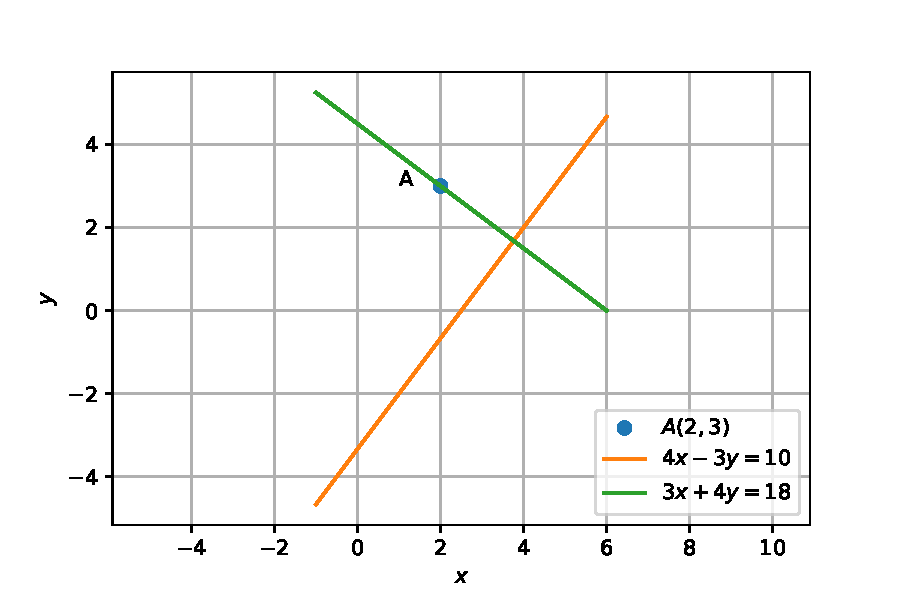
\includegraphics[width=\columnwidth]{./solutions/6/8/ExVIprob8.pdf}
    \caption{Solution}
    \label{eq:solutions/6/8/ExVIprob8.pdf}
\end{figure}




\end{enumerate}
